\documentclass{article}
\usepackage{ae,aecompl}
\usepackage{todonotes}
\usepackage{chngcntr}
\usepackage{tikz-cd}
\usepackage{graphicx}
\graphicspath{ {./images/}}
\usepackage[all,cmtip]{xy}
\usepackage{amsmath, amscd}
\usepackage{amsthm}
\usepackage{amssymb}
\usepackage{amsfonts}
\usepackage{bm}
\usepackage{qsymbols}
\usepackage{latexsym}
\usepackage{mathrsfs}
\usepackage{mathtools}
\usepackage{cite}
\usepackage{color}
\usepackage{url}
\usepackage{enumerate}
\usepackage{verbatim}
\usepackage[draft=false, colorlinks=true]{hyperref}
\usepackage{pdfpages}
\usepackage[margin=1.2in]{geometry}
\usepackage{IEEEtrantools}

\usepackage{fancyhdr}


\usepackage[nameinlink]{cleveref}


\DeclareMathOperator*{\ac}{accept}
\DeclareMathOperator*{\amax}{argmax}
\DeclareMathOperator*{\amin}{argmin}
\DeclareMathOperator*{\Aut}{Aut}
\newcommand {\al}{{\alpha}}
\newcommand {\abs}[1]{{\left\lvert#1\right\rvert}}
\newcommand {\A}{{\mathcal{A}}}
\newcommand {\AM}{{\mathrm{AM}}}
\newcommand {\AMp}{{\AM_{p}^{X}\!(\Ri_\w)}}
\newcommand {\B}{{\mathcal{B}}}
\DeclareMathOperator*{\Be}{Bern}
\newcommand {\Br}{{\dot{B}}}
\newcommand {\Ba}{{\mathfrak{B}}}
\newcommand {\C}{{\mathbb C}}
\newcommand {\ce}{\mathrm{c}}
\newcommand {\Ce}{\mathrm{C}}
\newcommand {\Cc}{\mathrm{C_{c}}}
\newcommand {\Ccinf}{\mathrm{C_{c}^{\infty}}}
\DeclareMathOperator{\cov}{Cov}
\DeclareMathOperator{\DEV}{DEV}
\newcommand {\Di}{{\mathbb D}}
\newcommand {\dom}{\mathrm{dom}}
\newcommand{\dist}{\stackrel{\mathrm{dist}}{=}}
\newcommand {\ud}{\mathrm{d}}
\newcommand {\ue}{\mathrm{e}}
\newcommand {\eps}{\varepsilon}
\newcommand {\veps}{\varepsilon}
\newcommand {\vrho}{{\varrho}}
\newcommand {\E}{{\mathbb{E}}}
\newcommand {\Ec}{{\mathcal{E}}}
\newcommand {\Ell}{L}
\newcommand {\Ellp}{{L_{p}[0,1]}}
\newcommand {\Ellpprime}{{L_{p'}([0,1])}}
\newcommand {\Ellq}{{L_{q}([0,1])}}
\newcommand {\Ellqprime}{{L_{q'}([0,1])}}
\newcommand {\Ellr}{L^{r}}
\newcommand {\Ellone}{{L_{1}([0,1])}}
\newcommand{\Elltwo}{{L_{2}([0,1])}}
\newcommand{\Ellinfty}{L^{\infty}}
\newcommand{\Ellinftyc}{L_{\mathrm{c}}^{\infty}}
\newcommand{\exb}[1]{\exp\left\{#1\right\}}
\DeclareMathOperator*{\Ext}{Ext}
\newcommand{\F}{{\mathcal{F}}}
\newcommand{\Fe}{{\mathbb{F}}}
\newcommand{\G}{{\mathcal{G}}}
\newcommand{\HF}{\mathcal{H}_{\text{FIO}}^{1}(\Rd)}
\newcommand{\Hr}{H}
\newcommand{\HT}{\mathcal{H}}
\newcommand{\ui}{\mathrm{i}}
\newcommand{\I}{{I}}
\newcommand{\J}{{\mathcal{J}}}
\newcommand{\id}{{\mathrm{id}}}
\newcommand{\iid}{\stackrel{\mathclap{\normalfont\mbox{iid}}}{\sim}}
\newcommand{\im}{{\text{im }}}
\newcommand{\ind}{{\perp\!\!\!\perp}}
\DeclareMathOperator*{\Int}{int}
\newcommand{\intx}{{\overline{\int_{X}}}}
\newcommand{\inte}{{\overline{\int_{\E}}}}
\newcommand{\la}{\lambda}
\newcommand{\rb}{\rangle}
\newcommand{\lb}{{\langle}}
\newcommand{\La}{\Lambda}
\newcommand{\calL}{{\mathcal{L}}}
\newcommand{\lp}{{\mathcal{L}}^{p}}
\newcommand{\lpo}{{\overline{\mathcal{L}}^{p}\!}}
\newcommand{\Lpo}{{\overline{\Ell}^{p}\!}}
\newcommand{\M}{{\mathbf{M}}}
\newcommand{\Ma}{{\mathcal{M}}}
\newcommand{\N}{{{\mathbb N}}}
\newcommand{\Na}{{{\mathcal{N}}}}
\newcommand{\norm}[1]{\left\|#1\right\|}
\newcommand{\normm}[1]{{\left\vert\kern-0.25ex\left\vert\kern-0.25ex\left\vert #1 
    \right\vert\kern-0.25ex\right\vert\kern-0.25ex\right\vert}}
\newcommand{\Om}{{{\Omega}}}
\newcommand{\one}{{{\bf 1}}}
\newcommand{\pic}{\text{Pic }}
\newcommand{\ph}{{\varphi}}
\newcommand{\Pa}{{\mathbb{P}}}
\newcommand{\Po}{{\mathcal{P}}}
\newcommand{\Q}{{\mathbb{Q}}}
\newcommand{\R}{{\mathbb R}}
\newcommand{\Rd}{{\mathbb{R}^{d}}}
\DeclareMathOperator{\rej}{reject }
\newcommand{\Rn}{{\mathbb{R}^{n}}}
\newcommand{\cR}{{\mathcal{R}}}
\newcommand{\Rad}{{\mathrm{Rad}}}
\newcommand{\ran}{{\mathrm{ran}}}
\newcommand{\Ri}{{\mathrm{R}}}
\newcommand{\supp}{{\mathrm{supp}}}
\newcommand{\Se}{\mathrm{S}}
\newcommand{\Sp}{S^{*}(\Rn)}
\newcommand{\St}{{\mathrm{St}}}
\newcommand{\Sw}{\mathcal{S}}
\newcommand{\T}{{\mathcal{T}}}
\newcommand{\ta}{{\theta}}
\newcommand{\Ta}{{\Theta}}
\newcommand{\topp}{\stackrel{p}{\to}}
\newcommand{\todd}{\stackrel{d}{\to}}
\newcommand{\toL}[1]{\stackrel{L^{#1}}{\to}} 
\newcommand{\toas}{\stackrel{a.s.}{\to}}
\DeclareMathOperator{\V}{Var}
\newcommand {\w}{{\omega}}
\newcommand {\W}{{\mathrm{W}}}
\newcommand {\Wnp}{\text{$\mathrm{W}$\textsuperscript{$n,\!p$}}}
\newcommand {\Wnpeq}{\text{$\mathrm{W}$\textsuperscript{$n\!,\!p$}}}
\newcommand {\Wonep}{\text{$\mathrm{W}$\textsuperscript{$1,\!p$}}}
\newcommand {\Wonepeq}{\text{$\mathrm{W}$\textsuperscript{$1\!,\!p$}}}
\newcommand {\X}{{\mathcal{X}}}
\newcommand {\Z}{{{\mathbb Z}}}
\newcommand {\Za}{{\mathcal{Z}}}
\newcommand {\Zd}{{\Z[\sqrt{d}]}}
\newcommand {\vanish}[1]{\relax}

\newcommand {\wh}{\widehat}
\newcommand {\wt}{\widetilde}
\newcommand {\red}{\color{red}}

% Distributions
\newcommand{\normal}{\mathsf{N}}
\newcommand{\poi}{\mathsf{Poisson}}
\newcommand{\bern}{\mathsf{Bernoulli}}
\newcommand{\bin}{\mathsf{Binomal}}
\newcommand{\multi}{\mathsf{Multinomial}}
\newcommand{\Exp}{\mathsf{Exp}}



% put your command and environment definitions here




% some theorem environments
% remove "[theorem]" if you do not want them to use the same number sequence


  \newtheorem{thrm}{Theorem}
  \newtheorem{lemma}{Lemma}
  \newtheorem{prop}{Proposition}
  \newtheorem{cor}{Corollary}

  \newtheorem{conj}{Conjecture}
  \renewcommand{\theconj}{\Alph{conj}}  % numbered A, B, C etc

  \theoremstyle{definition}
  \newtheorem{defn}{Definition}
  \newtheorem{ex}{Example}
  \newtheorem{exs}{Examples}
  \newtheorem{question}{Question}
  \newtheorem{remark}{Remark}
  \newtheorem{notn}{Notation}
  \newtheorem{exer}{Exercise}

\DeclareMathOperator{\med}{med}
\DeclareMathOperator{\sgn}{sgn}

\title{STATS305A - Lecture 18}
\author{John Duchi\\ Scribed by Michael Howes}
\date{11/30/21}

\pagestyle{fancy}
\fancyhf{}
\rhead{STATS305A - Lecture 18}
\lhead{11/30/21}
\rfoot{Page \thepage}

\begin{document}
\maketitle
\tableofcontents
\section{Announcements}
\begin{itemize}
    \item HW4 out today. There will be one multi-part question and one optional question.
    \item Etude 4 out tonight. Lots of the material for etude 4 will be covered in class on Thursday.
    \item Both will be due on Thursday next week at 5pm.
\end{itemize}
\section{M-estimation}
\subsection{Recap}
To do regression with M-estimators we use losses other than the squared error to measure error and fit models. For some loss $l:\R\to \R_+$ we solve the minimization problem
\[\text{minimize } \frac{1}{n}\sum_{i=1}^n l(y_i-x_i^Tb), \]
or sometimes
\[\text{minimize } \frac{1}{n}\sum_{i=1}^n l(y_i-x_i^Tb) + \text{Reg}(b). \]
Where $\text{Reg}(b)$ is some sort of regularizor like the norm of $b$. 
\subsection{Choosing the loss function}
In ordinary least squares we use the loss function $l(t) = \frac{1}{2}t^2$. There are two guiding principles we can use to choose alternative loss functions.
\begin{enumerate}
    \item Suppose that we could solve $\min_f \E[l(Y-f(X))]$ so that $f(x) = \amin_z \E[l(Y-z)|X=x]$. We would then like to choose the loss $l$ so that the function $f$ has a property that we care about. We will see this when we do quantile regression.
    \item Another approach is to choose a loss function $l$ so that we can avoid undue influence of outlying measurements/responses $y$. To do this we need a loss that is Lipschitz continuous. 
\end{enumerate}
\begin{defn}
    A loss function $l$ is \emph{Lipschitz} is there exists $C \ge 0$ such that for all $t,s\in \R$,
    \[\abs{l(t)-l(s)} \le C\abs{t-s}. \]
    The smallest such $C$ is called the \emph{Lipschitz constant} of $l$ and is denoted by $\norm{l}_{Lip}$.
\end{defn}
\begin{ex}
    The absolute error loss $l(t)=\abs{t}$ is Lipschitz with Lipschitz consant 1. We claim that $\amin_t \E[\abs{Y-t}]=\med(Y)$ where $\med(Y)$ denotes the median of $Y$. To see why this is true, let $R(t)=\E[\abs{Y-t}]$. We will compute the left and right derivates of $R$. Note that
    \[l'_{\leftarrow}(t)=\text{right derivative of $l$}=\sgn_+(t)=\begin{cases}
        1 &\text{if } t \ge 0,\\
        -1 &\text{if } t< 0.
    \end{cases}\]
    And
    \[l'_{\rightarrow}(t)=\text{left derivative of $l$}=\sgn_-(t)=\begin{cases}
        1 &\text{if } t > 0,\\
        -1 &\text{if } t\le 0.
    \end{cases}\]
    Thus
    \[R'_{\leftarrow}(t)=\E[\sgn_+(t-Y)]=\Pa(Y \le t)-\Pa(Y>t),\]
    and
    \[R'_{\rightarrow}(t)=\E[\sgn_-(t-Y)]=\Pa(Y <t)-\Pa(Y \ge t). \]
    Thus if $t < \med(Y)$, then $R'_{\to}(t) < 0$. If $t > \med(Y)$, then $R_{\leftarrow}(t) > 0$ and thus the minimizer of $R(t)$ is $\med(Y)$.
\end{ex}
\section{Outlier mitigation}
We will now talk more about guiding principle (b) which was about chosing losses that are robust against outliers. Define
\[L_n(b):= \frac{1}{n}\sum_{i=1}^n l(y_i-x_i^Tb). \]
We want to know what happens to the minimizer of $L_n(b)$ when we replace $(x_k,y_k)$ with $(x_k*, y_k^*)$. Let
\[L_{n,k}(b)=\frac{1}{n}\sum_{i \neq k} l(y_i-x_I^Tb)+\frac{1}{n}l(y_k^*-(x_k^*)^Tb). \]
Let $\wh{\beta}=\amin_b L_n(b)$ and let $\Delta_k = \amin_\Delta L_{n,k}(\wh{\beta}+\Delta)$.
\begin{prop}[Heuristic claim]
    If $l$ is Lipschitz, smooth and symmetric and the data is ``well-conditioned'', then $\Delta_k = O(1/n)$ (so $(x_k, y_k)$ has a small influence on $\wh{\beta}$).
\end{prop}
\begin{proof}[Sketch of proof]
    Note that $l$ being Lipschitz and differentiable implies that the derivates of $l$ are uniformly bounded by some constant $C$. Observe that
    \begin{align*}
        \nabla_{\Delta} L_{n,k}(\wh{\beta}+\Delta)&=\frac{1}{n}\sum_{i\neq k}l'(x_i^T(\wh{\beta}+\Delta)-y_i)x_i+\frac{1}{n}l'((x_k*)^T(\wh{\beta}+\Delta)-y_k^*)x_k^*\\
        &=\frac{1}{n}\sum_{i=1}^nl'(x_i^T(\wh{\beta}+\Delta)-y_i)x_i\\
        &~~~+\frac{1}{n}\left(l'((x_k*)^T(\wh{\beta}+\Delta)-y_k^*)x_k^*-l'(x_k^T(\wh{\beta}+\Delta)-y_k)x_k\right)\\
        &=\nabla_{\Delta} L_n(\wh{\beta}+\Delta)+\frac{1}{n}\left(C_k^*x_k^*-C_kx_k\right),
    \end{align*}
    where $C_k^*=l'((x_k*)^T(\wh{\beta}+\Delta)-y_k^*)$ and $C_k = l'(x_k^T(\wh{\beta}+\Delta)-y_k)$. We can do a Taylor's approximation of $\nabla_{\Delta} L_n(\wh{\beta}+\Delta)$ at $\Delta=0$. We know that $\nabla_{\Delta} L_n(\wh{\beta}+\Delta)\mid_{\Delta=0}=0$ since $\wh{\beta}$ minimizes $L_n(b)$. Thus
    \begin{align*}
        \nabla_{\Delta} L_{n,k}(\wh{\beta}+\Delta)&\approx \nabla^2 L_n(\wh{\beta})\Delta + \frac{1}{n}\left(C_k^*x_k^*-C_kx_k\right).
    \end{align*}
    If we set the right hand side equal to 0 we get
    \[ \Delta_k\approx \nabla^2 L_n(\wh{\beta})^{-1}\frac{1}{n}\left(C_k^*x_k^*-C_kx_k\right).\] 
    This gives the approximation since $l$ being Lipschitz implies that $C_k^*,C_k$ are bounded and $\{x_i\}_{i=1}^n$ being well-conditioned implies that the inverse Hessian $\nabla^2 L_n(\wh{\beta})^{-1}$ exists and isn't too wild.
\end{proof}
\begin{defn}
    The \emph{influence function} of an M-estimator is (roughly) the change in $\wh{\beta}^*$ when we change one observation. For M-estimators with $L(b)=\E[l(Y-X^Tb)]$ and $\beta^* =\amin_b L(b)$, we define the influence function $\psi$ to be
    \[\psi(x,y)=(\Delta^2 L(\beta^*))^{-1}l'(y-x^T\beta^*)x. \]
\end{defn}
\begin{thrm}
    Suppose $n \to \infty$. Let 
    \[\wh{\beta}(x,y)=\amin_b\left\{\sum_{i=1}^n l(y_i-x_i^Tb)+l(y-x^Tb)\right\},\]
    and
    \[\wh{\beta}=\amin_b\left\{\sum_{i=1}^n l(y_i-x_i^Tb)\right\}.\]
    Then, we have shown heuristically,
    \[\wh{\beta}(x,y)=\wh{\beta}+\frac{1}{n}\psi(x,y)+o(1/n).\]
\end{thrm}
The upshot is that if the derivative $l'(t)$ is bounded, then the estimator is robust. If $l'(t)$ is unbounded, then we the estimator is not robust. For example the following losses
\begin{align*}
    l_1(t)&=\log(1+e^t)+\log(1+e^{-t}),\\
    l_2(t)&=\abs{t}\\
    l_3(t)&=\begin{cases}
        \frac{1}{2}t^2 & \text{if } \abs{t}\le1,\\
        \abs{t}-\frac{1}{2} & \text{if } \abs{t}>1.
    \end{cases}
\end{align*}
have corresponding derivatives which are all bounded on $\R$
\begin{align*}
    l_1'(t)&=\frac{1}{1+e^{-t}}-\frac{1}{1+e^t},\\
    l_2'(t)&=\sgn(t)\\
    l_3'(t)&=\begin{cases}
        t & \text{if } \abs{t}\le1,\\
        \sgn(t) & \text{if } \abs{t}>1.
    \end{cases}
\end{align*}
The derivatives look like this with $l_1'$ in black, $l_2'$ in blue and $l_3'$ in red. Note that $l_2'$ and $l_3'$ overlap for $\abs{t} \ge 1$.
\begin{center}
    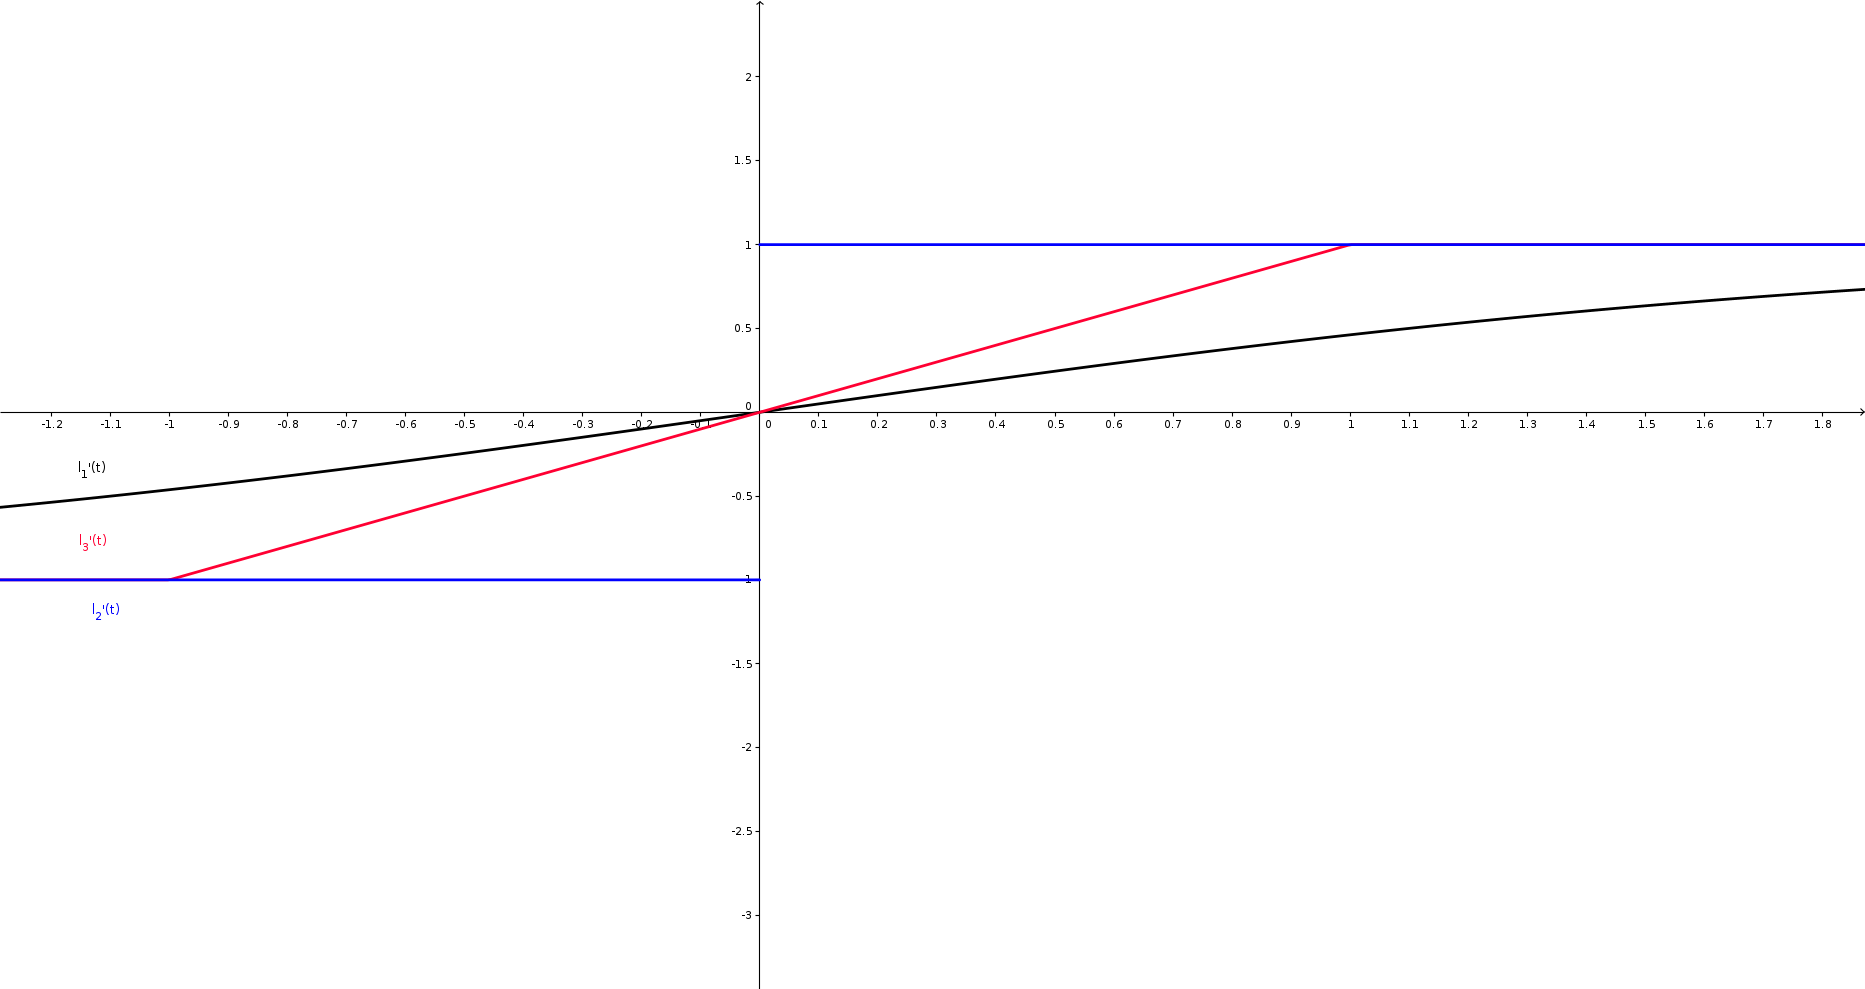
\includegraphics[width = \textwidth, trim = {0 5cm 0 2cm}, clip]{11_30_P01.png}
\end{center}
\section{Qunatile regression}
Often, instead of predicting $Y$, we want an interval where $Y$ is likely to be. That is, we would like a confidence set $\wh{c}(x)=[q_\al(x),q_{1-\al}(x)]$ such that $\Pa(Y \in \wh{c}(x)|X=x)=1-2\al$ (this is impossible but let's try anyway). There are many applications where we are more interested in $\wh{c}(x)$ than $\wh{y}$. For example we might be
\begin{itemize}
    \item Predicting election results,
    \item Predicting patient survival times,
    \item Predicting air quality.
\end{itemize}
What loss should we choose to get something like this? We could fit two (or more) models that predict the $\al$, $1-\al$ quantiles of $Y|X=x$. To do this we use the \emph{pinball loss} (also called the quantile loss). For $\al \in (0,1)$, let $l_\al$ be the loss function given by
\[l_\al(t)=\al(t)_++(1-\al)(-t)_+, \]
where $(t)_+=\max{0,t}$ so that $(t)_+=0$ for $t \le 0$ and $(t)_+=t$ for $t\ge 0$. The function $l_\al$ looks something like this. The blue loss is typical for $\al > 1/2$ and the black loss is typical for $\al < 1/2$. 
These losses are chosen with guiding principle (a) in mind. We will now show that the minimizers of $\E[l_\al(Y-t)]$ are $\al$-quanties of $Y$.
\begin{center}
    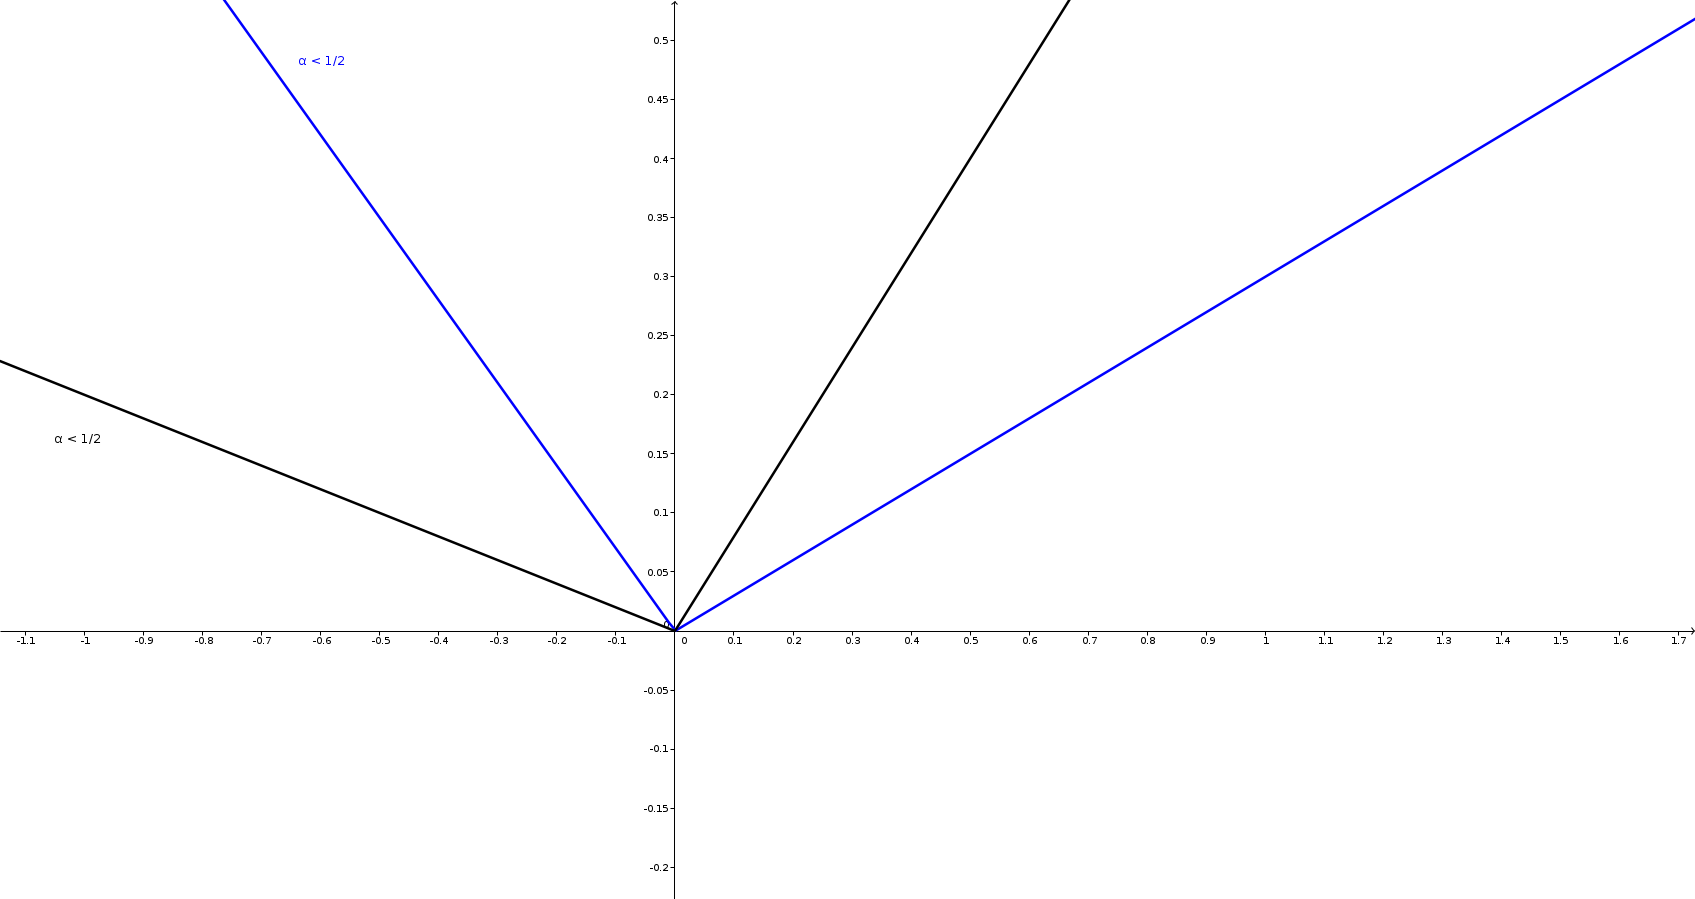
\includegraphics[width = 0.7\textwidth, trim = {0 1cm 3cm 0}, clip]{11_30_P02.png}
\end{center} Define $R_\al(t)=\E[l_\al(Y-t)]$, then
\[R_\al'(t)=\E[-\al\one(Y >t)+(1-\al)\one(Y \le t)]=(1-\al)\Pa(Y \le t)-\al\Pa(Y >t).\]
If $\Pa(Y \le t)>\al$, then $\Pa(Y > t) < 1-\al$ and $R'_\al(t) > 0$ so $t$ is too large. If $\Pa(Y \le t)< \al$, then $\Pa(Y > t)>1-\al$ and $R'_\al(t)<0$ so $t$ is too small. Thus
\[\amin_t R_\al(t)=\inf\{t:\Pa(Y \le t) \ge \al\} = \al\text{-quantile of $Y$}.\]
\emph{Quantile regression} is the following procedure. For $\al \in (0,1/2)$, fit two models 
\[\wh{\beta}_\al = \amin_b \sum_{i=1}^n l_\al(y_i-x_i^Tb)~~~\text{and}~~~ \wh{\beta}_{1-\al} = \amin_b\sum_{i=1}^n l_{1-\al}(y_i-x_i^Tb).\]
Then our prediction intervals are 
\[\wh{c}(x)=[\wh{\beta}_\al^T x, \wh{\beta}_{1-\al}^Tx].\]
More generally, instead of linear functions we could consider fitting $f \in \F$ where $\F$ is some function class. We would then have
\[\wh{f}_\al = \amin_{f\in\F} \sum_{i=1}^n l_\al(y_i-f(x_i))~~~\text{and}~~~ \wh{f}_{1-\al} = \amin_{f\in \F}\sum_{i=1}^n l_{1-\al}(y_i-f(x_i)).\]
We would then again define
\[\wh{c}(x)=[\wh{f}_\al(x), \wh{f}_{1-\al}(x)]. \]
Some issues:
\begin{itemize}
    \item There is no guarantee that $\wh{f}_\al(x) \le \wh{f}_{1-\al}(x)$. We can fix this by defining
    \[\wh{c}(x)=[\min\{\wh{f}_\al(x), \wh{f}_{1-\al}(x)\},\max\{\wh{f}_\al(x), \wh{f}_{1-\al}(x)\}]. \]
    \item We do not have any gaurantee that $\wh{c}(x)$ is a valid confidence interval for $Y$ given $X=x$. That is we have no reason to believe that
    \[\Pa(Y \in \wh{c}(x)|X=x)=1-\al. \]
\end{itemize}
The second issue cannot be resolved. It is a \underline{fact} that without strong assumptions, you cannot have \emph{conditional converage}. That is we cannot find a procedure $\wh{c}$ based on a i.i.d. sample $\{x_i,y_i\}_{i=1}^n$ such that 
\[\Pa(Y_{n+1}\in \wh{c}(x_{n+1})|X_{n+1}=x_{n+1})=1-\al+o(1), \]
where $Y_{n+1},x_{n+1}$ is a new independent date point from the same distribution as our sample. 

We can achieve \emph{marginal coverage}. That is the exists a procedure $\wh{c}$ such that 
\[\Pa(Y_{n+1}\in \wh{c}(X_{n+1}))\ge 1-\al. \]
Furthermore if $Y$ is continuous, then we can find $\wh{c}$ such that 
\[\Pa(Y_{n+1} \in \wh{c}(X_{n+1})) = 1-\al \pm \frac{1}{n}. \]
These ideas will be discussed on Thursday when we look at conformal confidence intervals. 
\end{document}